\chapter{Sustainability Strategy}
\label{ch:sustainability}

In light of the pressing environmental challenges, adopting sustainable practices in the aviation industry is crucial.
Although significant advancements in aircraft efficiency have been achieved over recent decades, the tenfold surge in air traffic has led to a rise in CO$_2$ emissions~\cite{SUPAEROCO2}, as illustrated in \Cref{fig:co2}.
As new urban mobility solutions develop, it is essential that the progress of Urban Air Mobility (UAM) does not compromise the health and well-being of our planet.
Therefore, it is vital to acknowledge that the choices made in the design, manufacturing, and operation of aircraft have extensive environmental impacts, affecting communities and future generations.

\begin{figure}[ht]
    \centering
    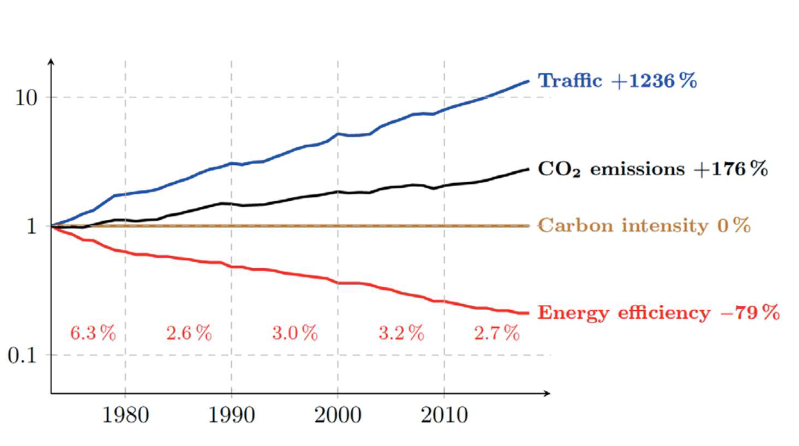
\includegraphics[width=0.6\linewidth]{figures/AviationEmissions.png}
    \caption{Factors in aircraft CO2 emissions, from Scott Delbecq et al. \cite{SUPAEROCO2}}
    \label{fig:co2}
\end{figure}



For this reason, a sustainability development strategy has been formulated at the initial stages of the project.
This strategy has its foundations in the three categories of sustainability: social, economic, and environmental~\cite{baselinerepo}.
The plan also sets the basis for a sustainable team, focused on the principles of adaptability, trust, transparency, and contribution~\cite{ProjectPlan}.
In this section, the way through which sustainability is ensured during the design process is explained.
This begins with the trade-off criteria selected for decision-making and continues with considerations such as material choices.

\section{A Sustainable Trade-Off}
One’s commitment to sustainability shall be established prior to initiating the design or project, as it can influence decisions made in the very early development stages.
The inclusion of sustainability-related criteria in the trade-off is essential to choose a configuration that achieves the best results possible.
Some configurations might be inherently more sustainable than others.
In the trade-off, as described previously, ground footprint, transition effectiveness, noise footprint, and energy efficiency were considered for the evaluation of each possible design.
As a lot more criteria contributed to the final choice, it should be analysed how the winning design concept, the rotating wing, performs in terms of sustainability with respect to the other concepts.
To do so, the sustainable criteria and sub-criteria are considered, multiplied by their respective weight, and summed up.
This procedure yields the results shown in \Cref{tab:sustevaluation}:


\begin{table}[ht]
\centering
\caption{Sustainability performance of the designs (maximum score is 2.88)}
\label{tab:sustevaluation}
\begin{tabular}{c|c|c|c}
\toprule
\textbf{\ref{C1.5}}                          &~\textbf{\ref{C2.1}}                          &~\textbf{\ref{C2.6}}                          &~\textbf{\ref{C2.10}}                         \\ \bottomrule
 \cellcolor[HTML]{E0E383}1.70 & \cellcolor[HTML]{A2D07F}2.33 & \cellcolor[HTML]{E0E383}1.70 & \cellcolor[HTML]{FCBF7B}1.15 \\ \toprule
\end{tabular}
\end{table}

Given the scores shown in \Cref{tab:sustevaluation}, concept \ref{C2.1}, the design choice, was considered the most sustainable option of the four.
This was a further confirmation of the consistency of the trade-off criteria weights distribution, allowing sustainability performance not to lose importance overall.

Now that the trade-off has been performed and the final design chosen, general considerations will be made and design choices suggested. At this preliminary stage, these considerations are not intended to be constraining. However, every effort will be made to ensure they are followed to a reasonable extent.

\section{Sustainable Materials Selection}
Material selection activities occur throughout nearly all phases of product development, with a significant focus during the preliminary stages where the product concept is defined.
Environmental analysis of the product typically takes place during the detailed phase of the design.
This analysis includes assessing the environmental impact and the availability of raw materials, as illustrated in \Cref{fig:materialsSelection}.


\begin{figure}[ht]
    \centering
    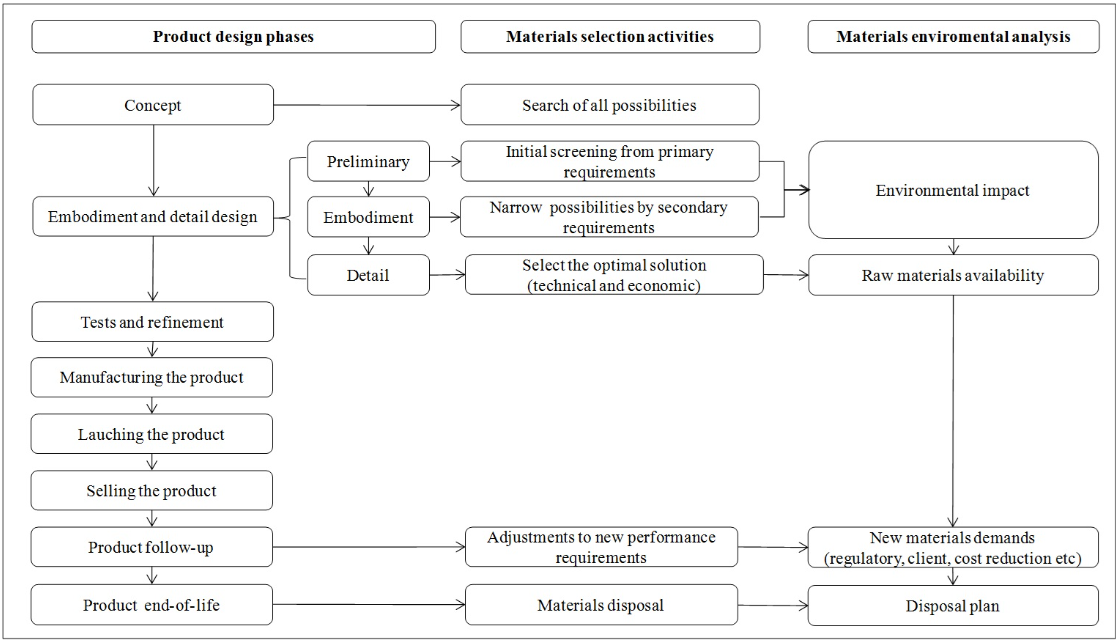
\includegraphics[width=0.9\linewidth]{figures/MaterialSelection.png}
    \caption{Selection activities and environmental analysis of materials in the product design \cite{santos2016materials}}
    \label{fig:materialsSelection}
\end{figure}

Before searching for possible material solutions or making any kind of decision, it is important to realise what aspects are important for the choice of a sustainable material. It is important to consider sustainability indicators that encompass environmental, economic, and social dimensions, reflecting their influence throughout the product's entire life cycle, as shown in \cref{fig:ecoindicators}.
Creating a comprehensive eco-indicator for each material, which encapsulates all environmental impacts, is difficult.
As a result, materials selection strategies often prioritise impacts in specific phases of the product life cycle.
For instance, the Ashby Eco-Audits analytical methodology~\cite{ashby2012materials} emphasises evaluating energy consumption and carbon footprint impacts at different stages of the product's life.
However, social and economic eco-indicators should not be neglected.

\begin{figure}[ht]
    \centering
    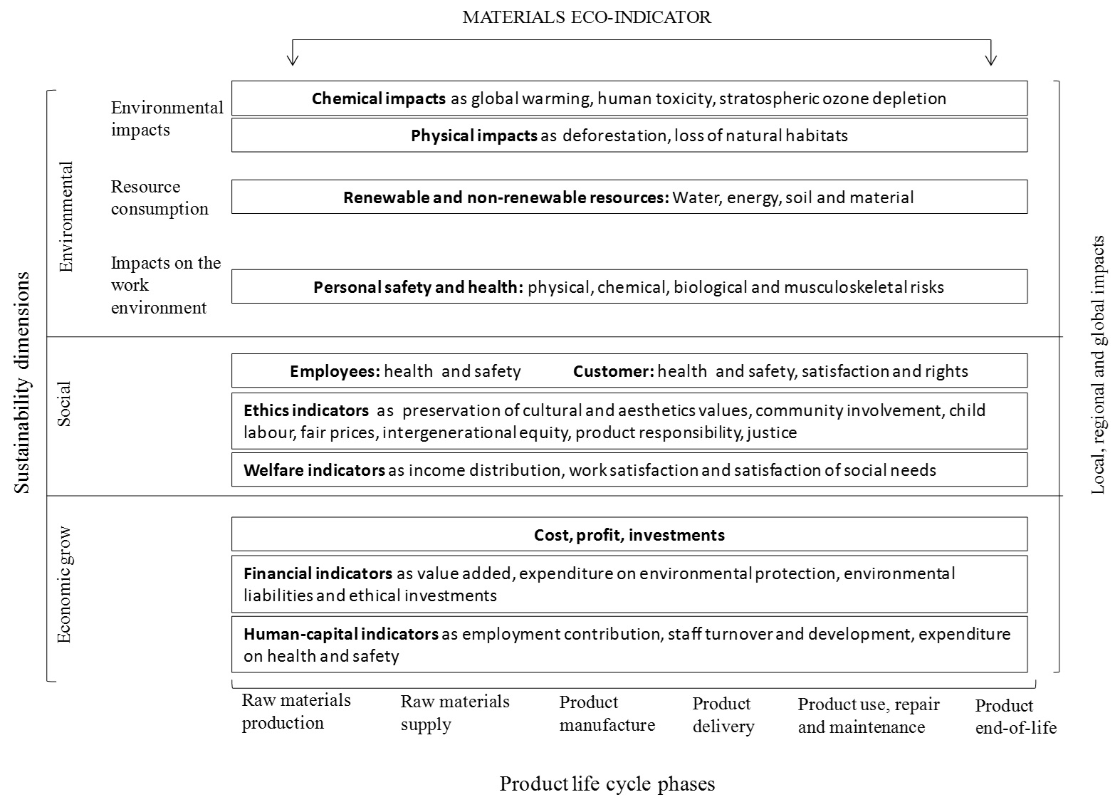
\includegraphics[width=0.9\linewidth]{figures/EcoIndicators.png}
    \caption{Materials eco-indicator determined by its impact on the product life cycle phases \cite{santos2016materials}}
    \label{fig:ecoindicators}
\end{figure}


When thinking of engineering projects, one would mainly focus on the choice of materials for structural components.
Although great improvements have been made in the field, often the options are limited due to structural reasons.
Realising how the interior design of the cabin, subject to fewer constraints, allows for a bigger margin of improvements is essential.
Furthermore, as Santos et al. \cite{santos2016materials} underline, this often gains a competitive advantage as a possible marketing solution, especially in the context of private vehicles.

\section{Life-time \& Reusability}
Realising how the reusability of the design is going to be approached is considered crucial for the project.
Its importance is highlighted by the presence of requirements Co-4-STK13-1-5 (\Cref{tab:reqtradeoff}) and Co-4-STK13-1-6, where the latter reads as follows: the vehicle structure shall be reusable for at least 10 years after its life.

Different aspects need to be considered during the design in order to ensure compliance with these requirements.
The following factors are to be considered:
\begin{itemize}
    \item \textbf{Modularity:} Creating a modular structure allows for easy disassembly and reassembly of components.
    This facilitates repairs, upgrades, and repurposing of parts, extending the vehicle’s lifespan.
    \item \textbf{Standardisation:} Implement standardised components and interfaces to ensure compatibility with future technologies and systems.
    This simplifies the integration of new features over time.
\end{itemize}

Additionally, End-Of-Life (EOL) aircraft processing is a problem that poses technological and environmental challenges.
The EOL processing includes four major steps: decontamination, disassembly of parts, dismantling of the remaining carcass, materials’ recovery and/or landfill.
The disassembly of reusable parts is a selective and non-destructive process.
Aspects of the graphical method, wave propagation approach, and Petri nets approach in disassembly applications are considered by \textcite{camelot2013decision} to support different strategies to perform a disassembly and guarantee collaboration between technicians.

By integrating these considerations into the design process, an eVTOL with a reusable structure that meets sustainability goals and ensures long-term viability can be designed.

\section{Sustainable Objectives of UAM}
Last but not least, it is important to acknowledge what the sustainable objectives of Urban Air Mobility are.
Air taxis are indeed designed for short-distance trips and are not meant to substitute aircraft.
One significant advantage of air taxis is their potential to reduce the number of vehicles on the road, thereby reducing traffic congestion and translating some of it to the skies.
This could lead to a decrease in noise and carbon emissions from ground vehicles, promoting cleaner urban environments.

As also highlighted by Arbin Instruments~\cite{UAMSust}, the extensive infrastructure needed for the adoption of electric public transport makes them a major undertaking for larger cities.
 In contrast, eVTOLs only require transportation hubs, eliminating the need for additional roads or tracks.

%\textbf{Energy Efficiency}: Energy efficiency should be prioritised in all design aspects, including propulsion systems, avionics, and auxiliary systems. Lightweight structures, aerodynamic design principles, and efficient propulsion technologies will be utilised to maximise energy efficiency and minimise emissions during operations.

%\textbf{Renewable Energy Integration}: Opportunities to integrate renewable energy sources, such as solar or wind power, into the operation and charging infrastructure of the eVTOL will be explored. This can help reduce reliance on fossil fuels and decrease greenhouse gas emissions associated with charging and operation.

%\textbf{Materials \& Manufacturing}: Materials manufacturing processes differ widely, thus the environmental impact of manufacturing processes and their emissions will be considered for the material selection. Trade-offs will be performed for the choice of materials for the different structures. In these trade-offs, the extraction and processing emissions of these materials will be accounted for. 

%\textbf{Recyclability and End-of-Life Management}: The eVTOL will be designed with recyclability in mind, selecting materials that are recyclable at the end of the aircraft's life cycle. A program or partnership with recycling facilities can be implemented to ensure responsible disposal and recycling of components and materials. A plan will be drafted for a ten-year usage of the various components of the vehicle. 

%\textbf{Noise Reduction}: Design features to minimise the noise footprint of the eVTOL during operation. This can mitigate the environmental impact on local communities and ecosystems, particularly in urban environments.

%\textbf{Supply Chain Sustainability}: Working with suppliers and partners who have already targeted sustainability throughout the supply chain, from raw material extraction to component manufacturing. Factors such as ethical sourcing, fair labour practices, and minimal transportation-related emissions in supplier selection and procurement decisions will be considered.

%\textbf{Regulatory Compliance and Certification}:  Multiple European institutions have drawn up regulations and standards to preserve the environment and slow the global warming process. Compliance with applicable environmental regulations and standards throughout the design will be ensured. 

%The elements outlined above primarily focus on how the design team intends to position the product within a market that prioritises sustainability. However, sustainability can also be integrated into the design process itself by considering additional factors such as:

%\textbf{New Design vs COTS}: In the design phase, there are frequent decisions regarding whether to pursue a newly designed, more efficient, and environmentally friendly product or to opt for Commercial Off-The-Shelf (COTS) solutions. While new designs hold promise, they often entail testing and certification processes, potentially leading to a significant waste of resources. When confronted with this dilemma, the design team will undertake a thorough evaluation of both options before reaching a decision.

%\textbf{Toxicity of Materials:} In the design process, the use of non-toxic materials to minimise environmental impact and safeguard the well-being of personnel involved in manufacturing and operations is prioritised. By choosing less harmful substances, create a safer working environment and mitigate the risk of occupational hazards. This approach extends throughout the product life-cycle, promoting sustainability and resilience in our operations.

%It is important to consider how people impact the sustainability of a project, not just the design itself. As already mentioned in the project planning phase, the following major principles have been selected to guide the team dynamics: \textbf{Adaptability }(being able to adapt, learn new skills, and face unexpected challenges); \textbf{Trust}: creating a safe and pleasurable work environment, with easiness of cooperation; \textbf{Transparency}: communicating with the rest of the group about one's work, accessibility of information must be facilitated; \textbf{Contribution}(willingness to contribute to the project, help others, and respect the schedule and deadlines).

%These values, alongside the guidelines that stem from them, constitute the backbone for a sustainable work environment and the creation of a so-called \enquote{sustainable team}. The same pillars should however translate also to the public image of the product and the team's relations with subcontractors. 

%In addition to the sustainability development plan, requirements have been established in \Cref{tab:constrreqfinal} concerning sustainability.
%These were specifically drawn to meet the needs of certain stakeholders such as environmental organisations (\ref{stk:environmental-orgs}) and the EU government (\ref{stk:EU}). Local regulations regarding sustainability may also apply depending on the country or municipality.

%Now that the key elements of the sustainability development strategy have been outlined, a technique used for the evaluation of the level of sustainability of the result shall be described. A Life Cycle Assessment constitutes a valuable tool in this regard. 

%It is thus considered essential to conduct a comprehensive LCA to quantify the environmental impacts of the design from raw material extraction to manufacturing, use, and disposal. This involves assessing factors such as energy consumption, greenhouse gas emissions, water usage, and waste generation. Together with this, use will be made of specific metrics to quantify environmental performance, such as carbon footprint, water footprint, and ecological footprint. These metrics provide quantitative measures of the design's environmental impact and allow for comparison with benchmarks or targets.

%Considerations such as labour rights, health and safety, community engagement, and social equity would be valuable to implement in order to evaluate the social impact of the design on stakeholders, communities, and workers involved in the design, manufacturing, and operation processes. However, they are deemed too out of the scope of the project, and they will be considered only to a limited extent.

